\hspace{-0.6mm}[12~v\textsuperscript{o}] et fac, ut fila pro dioptris in eorum focis se intersecent ad crucem, ita ut utraque possint esse in debita ab oculo distantia, introspiciendo per foramen laterale, inde aperiendo tubos super dicta junctura ad aliquem angulum et introspiciendo per foramen laterale, distingues planissime, una eademque opera duo objecta, tubis directe illata, et ad oculum reflexa. \makebox[1.0\textwidth][s]{Haec ut clarius intelligantur, addatur delineatio eorum in plano. Fac ut \textit{aabb} in figura}
\pend
\vspace{1.2em}
\count\Afootins=1200
\count\Bfootins=1200
\count\Cfootins=1200
\begin{center}   
\centering                 
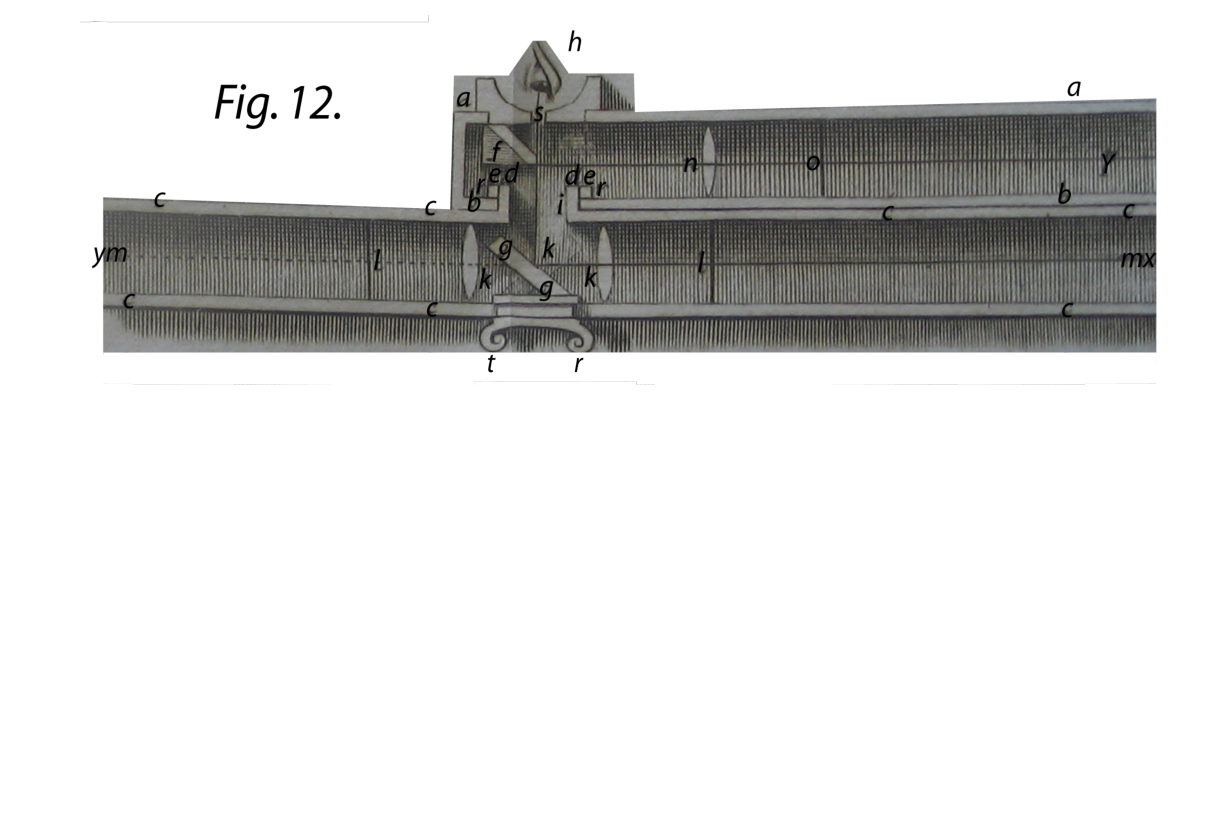
\includegraphics[trim = 0mm 1mm 0mm 2mm, clip, width=1.0\textwidth]{images/LH0351506_012v-dext12.pdf}\newline
\vspace*{3mm}\centering[\textit{Fig. 3; erg. Hrsg. nach Hooke Fig. 12}]
\end{center}
\pstart\noindent 12\textsuperscript{ma} 
\edtext{}{
%{\lemma{figura 12\textsuperscript{ma}}\Cfootnote{An dieser Stelle im Manuskript freigelassene Fl\"{a}che, vermutlich um die im Text besprochene Figur aus \textsc{R. Hooke??}, \textit{Animadversions??}, S. xx einf\"{u}gen.}}
\lemma{}\Bfootnote{12\textsuperscript{ma} \textbar\ 12\textsuperscript{ma} \textit{streicht Hrsg.} \textbar\ repraesentet \textit{L}}} repraesentet superiorem et \textit{cc} inferiorem \edtext{Tubum. Fac \textit{dd} repraesentet eam partem}{\lemma{inferiorem}\Bfootnote{\textit{(1)}\ Tubi partem. \textit{(2)}\ Tubum. [...] partem \textit{L}}} juncturae quae ad inferiorem Tubum pertinet, ad unum extremum, \edtext{per quod}{\lemma{extremum,}\Bfootnote{\textit{(1)}\ ubi \textit{(2)}\ per quod \textit{L}}} inter se junguntur (tubi), et aperiri possit per modum sectoris. \textit{i} repraesentet cavum vel \edtext{centrum juncturae,}{\lemma{}\Bfootnote{centrum \textbar\ juncturae \textit{streicht Hrsg.} \textbar\ juncturae, \textit{L}}} quo communicant cavitates duorum Tuborum. \textit{ec} repraesentet partem dictae juncturae quae pertinet ad superiorem Tubum, quae non est nisi foramen per latus inferius, crassum satis, \textit{to incompass} (inserendo) \textit{the cylinder dd of the lower tube,}\edtext{}{\lemma{\textit{tube},}\Cfootnote{a.a.O., S. 57.}} \textit{rr} repraesentet \textit{plate}\edtext{}{\lemma{\textit{plate}}\Cfootnote{a.a.O., S. 57.}}, (laminam) accochleatam, quae partes juncturae tenet firmas \textit{instead of rivetting.}\edtext{}{\lemma{\textit{rivetting}.}\Cfootnote{a.a.O., S. 57.}} \textit{s} repraesentet cavitatem in latere, qua oculus \textit{h} inspicit, et \textit{f} metallum reflexivum in superiore Tubo, \textit{reaching only half way the tube,}\edtext{}{\lemma{\textit{tube},}\Cfootnote{a.a.O., S. 57.}} et \textit{gg} metallum reflexivum in inferiore \textit{reaching over the whole cavity}\edtext{}{\lemma{\textit{cavity}}\Cfootnote{a.a.O., S. 57.}}. Inde \textit{n. o. p.} repraesentabunt oculare\protect\index{Sachverzeichnis}{ocular} vitrum, fila dioptrica, et vitrum objectivum superioris Tubi, et \textit{k. l. m.} eadem in inferiore; et quem\-cunque angulum invicem faciant Tubi; tantisper dum aperti sunt super dicta junctura, oculus \textit{h} introspiciens in \textit{s} directe \edtext{inspiciet per axem utrique}{\lemma{inspiciet}\Bfootnote{\textit{(1)}\ axem utriusque \textit{(2)}\ per axem utrique \textit{L}}}, et videbit fila dioptrica directe ad crucem secantia, puncta objectorum, quorum mensurantur distantiae. Unde facile intelligitur modus quo quadranti\protect\index{Sachverzeichnis}{quadrans} nostro supra descripto ista possint applicari[,] tantum enim supponatur \textit{cc}. Superius latus, inferioris Tubi repraesentare \textit{the fixt side arm of the} \edtext{\textit{quadrant\protect\index{Sachverzeichnis}{quadrans},}}{\lemma{\textit{quadrant},}\Cfootnote{a.a.O., S. 57.}} \edtext{et}{\lemma{\textit{quadrant},}\Bfootnote{\textit{(1)}\ cum \textit{(2)}\ et \textit{L}}} \textit{dd} junctura nostra, repraesentabit \textit{dd} juncturam quadrantis\protect\index{Sachverzeichnis}{quadrans}, et \textit{bb}, inferius latus superioris Tubi repraesentabit brachium quadrantis\protect\index{Sachverzeichnis}{quadrans} mobile et applicando duos Tubos ad has partes, caeteraque aptando, res erit facta. Hic Tubus serviet ad sumendum angulum quemlibet, qui non sit major quadrante\protect\index{Sachverzeichnis}{quadrans}. Sed pro majoribus angulis varianda nonnihil constructio est; cujus nunc subjiciam descriptionem. Nimirum primum tubi duplicis longitudinis priorum id est tam longi ante quam post centrum, vitrum reflexivum ita fiat, ut sit \edtext{rotunde circumactum}{\lemma{rotunde}\Bfootnote{\textit{(1)}\ tornatum \textit{(2)}\ circumactum \textit{L}}}, et reflectat radios exacte retrorsum, ut antea prorsum: inde fixetur in altero dimidio Tubi dioptra\protect\index{Sachverzeichnis}{dioptra} Telescopica\protect\index{Sachverzeichnis}{telescopium}, ut duae superiores, inde \edtext{accommoda, ut}{\lemma{}\Bfootnote{accomoda \textbar\ , ut \textit{streicht Hrsg.} \textbar\ , ut \textit{L}}} possit videri prorsum et retrorsum, quo facto facile intelliget Lector, quomodo quivis angulus sumi possit, ad ipsam usque magnitudinem duorum angulorum rectorum. Satis enim planum est, duos tubos supra descriptos applicatos ad quadrantem\protect\index{Sachverzeichnis}{quadrans}, mensurare quemlibet angulum usque ad quadrantem\protect\index{Sachverzeichnis}{quadrans} seu 